\documentclass[12pt,a4paper]{report}
\setlength\textwidth{145mm}
\setlength\textheight{247mm}
\setlength\oddsidemargin{15mm}
\setlength\evensidemargin{15mm}
\setlength\topmargin{0mm}
\setlength\headsep{0mm}
\setlength\headheight{0mm}

\usepackage[utf8]{inputenc}
\usepackage{graphicx}
\usepackage{epstopdf}
\usepackage{amsthm}
\usepackage{appendix}
\usepackage{nomencl}
\usepackage{parskip}
\usepackage{listings}
\usepackage{enumitem}
\usepackage{nameref}

\makenomenclature

% Scala listing.
\lstdefinelanguage{Scala}{
  morekeywords={abstract,case,catch,class,def,%
    do,else,extends,false,final,finally,lazy,%
    for,if,implicit,import,match,mixin,%
    new,null,object,override,package,%
    private,protected,requires,return,sealed,%
    super,this,throw,trait,true,try,%
    type,val,var,while,with,yield},
  otherkeywords={=>,<-,<\%,<:,>:,\#,@},
  sensitive=true,
  morecomment=[l]{//},
  morecomment=[n]{/*}{*/},
  morestring=[b]",
  morestring=[b]',
  morestring=[b]"""
}
\lstset{language=Scala}

% JavaScript listing.
\lstdefinelanguage{JavaScript}{
  keywords={break, case, catch, continue, debugger, default, delete, do, else, finally, for, function, if, in, instanceof, new, return, switch, this, throw, try, typeof, var, void, while, with},
  morecomment=[l]{//},
  morecomment=[s]{/*}{*/},
  morestring=[b]',
  morestring=[b]",
  sensitive=true
}

% Less indented chapter titles.
\makeatletter
\def\@makechapterhead#1{
  {\parindent \z@ \raggedright \normalfont
   \Huge\bfseries \thechapter. #1
   \par\nobreak
   \vskip 20\p@
}}
\def\@makeschapterhead#1{
  {\parindent \z@ \raggedright \normalfont
   \Huge\bfseries #1
   \par\nobreak
   \vskip 20\p@
}}
\makeatother

% Chapter without a number but still in the table of contents.
\def\chapwithtoc#1{
\chapter*{#1}
\addcontentsline{toc}{chapter}{#1}
}

\begin{document}

\lefthyphenmin=2
\righthyphenmin=2



%%%%%%%%%%%%%%%%%%%%%%%%%%%%%%%%%%%%%%%%%%%%%%%%%%%%%%%%%%%%%%%%%%%%%%%%%%%%%%%%
\pagestyle{empty}

\begin{center}
\large Charles University in Prague
\medskip

Faculty of Mathematics and Physics

\vfill

{\bf\Large MASTER THESIS}

\vfill

\centerline{\mbox{\includegraphics[width=60mm]{img/Logo.eps}}}

\vfill

\vspace{5mm}

{\LARGE Jan Široký}

\vspace{15mm}

{\LARGE\bfseries Scala Web Application Toolkit}

\vfill

Department of Distributed and Dependable Systems

\vfill

\begin{tabular}{rl}
Supervisor of the master thesis: & Pavel Ježek \\
\noalign{\vspace{2mm}}
Study programme: & Computer Science \\
\noalign{\vspace{2mm}}
Specialization: & Software Systems \\
\end{tabular}

\vfill

Prague 2013
\end{center}



%%%%%%%%%%%%%%%%%%%%%%%%%%%%%%%%%%%%%%%%%%%%%%%%%%%%%%%%%%%%%%%%%%%%%%%%%%%%%%%%
\newpage
\noindent 
Dedication.



%%%%%%%%%%%%%%%%%%%%%%%%%%%%%%%%%%%%%%%%%%%%%%%%%%%%%%%%%%%%%%%%%%%%%%%%%%%%%%%%
\newpage

\vglue 0pt plus 1fill
\noindent
I declare that I carried out this master thesis independently, and only with the cited sources, literature and other professional sources.

\medskip\noindent
I understand that my work relates to the rights and obligations under the Act No. 121/2000 Coll., the Copyright Act, as amended, in particular the fact that the Charles University in Prague has the right to conclude a license agreement on the use of this work as a school work pursuant to Section 60 paragraph 1 of the Copyright Act.

\vspace{10mm}
\hbox{\hbox to 0.5\hsize{%
In ........ date ............
\hss}\hbox to 0.5\hsize{%
signature of the author
\hss}}
\vspace{20mm}



%%%%%%%%%%%%%%%%%%%%%%%%%%%%%%%%%%%%%%%%%%%%%%%%%%%%%%%%%%%%%%%%%%%%%%%%%%%%%%%%
\newpage

\vbox to 0.5\vsize{
\setlength\parindent{0mm}
\setlength\parskip{5mm}

Název práce: 
Scala Web Application Toolkit

Autor: 
Jan Široký

Katedra: 
Katedra distribuovaných a spolehlivých systémů

Vedoucí diplomové práce: 
Mgr. Pavel Ježek Ph.D, Katedra distribuovaných a spolehlivých systémů

Abstrakt:
TODO

Klíčová slova:
Scala, JavaScript, RIA, JSON, RPC

\vss}\nobreak\vbox to 0.49\vsize{
\setlength\parindent{0mm}
\setlength\parskip{5mm}

Title:
Scala Web Application Toolkit

Author:
Jan Široký

Department:
Department of Distributed and Dependable Systems

Supervisor:
Mgr. Pavel Ježek Ph.D, Department of Distributed and Dependable Systems

Abstract:
TODO

Keywords:
Scala, JavaScript, RIA, JSON, RPC

\vss}



%%%%%%%%%%%%%%%%%%%%%%%%%%%%%%%%%%%%%%%%%%%%%%%%%%%%%%%%%%%%%%%%%%%%%%%%%%%%%%%%
\newpage
\pagestyle{plain}
\setcounter{page}{1}
\tableofcontents



%%%%%%%%%%%%%%%%%%%%%%%%%%%%%%%%%%%%%%%%%%%%%%%%%%%%%%%%%%%%%%%%%%%%%%%%%%%%%%%%
\chapter{Introduction}

The environment of websites and web applications has been rapidly evolving and going through a lot of changes for the last twenty years. It may even be considered the most dynamic area of software development, currently together with mobile application development. The first websites were just static HTML pages linked together with anchors. But people soon found out it is possible to generate the pages on the server, thus provide a dynamic behavior and mimic standard desktop applications. The obvious drawback is that after every action of the user, the whole page has to be reloaded. 

In order to mitigate the problems of dynamic pages, new browser based technologies started to emerge, the most known are Flash\cite{Flash}, Java Applets\cite{JavaApplets} and JavaScript\cite{JavaScript}\cite{EcmaScript}. The proprietary Flash and Java Applets were designed solely for the purpose of web application development, JavaScript was in the first phases meant as a simple scripting language for manipulation with the page. However with the ability to send HTTP requests (known as AJAX\cite{Ajax}), it turned out that JavaScript may be even used as a platform for web applications. 

The current tendency is to move from the proprietary technologies to JavaScript, which is widely supported by browsers and devices. With the new HTML5\cite{Html5} specifications, which are being adopted quite quickly by the major browsers, even the advantages of other technologies (e.g. video in Flash) are disappearing. So a growing number of web applications is in the moment designed as a single HTML page with embedded JavaScript that takes care of everything. And the single page is backed by a server API that the client JavaScript communicates with. This architecture is actually quite similar to the desktop applications, so design patterns and techniques that are already proven-right from the desktop environment may be utilized. From the architectural point of view, the web and desktop application branches are merging.

During past couple of years, JavaScript has been used so extensively, that developers started to reach its limits in modularization and maintainability, mainly while working on big applications. Other programming languages however handle those issues better and because JavaScript is a rather powerful programming language, it is not that difficult to use it as a compilation target for those languages. Even completely new programming languages with the only purpose to improve JavaScript appeared, so currently there is more than one hundred of languages that compile to JavaScript\cite{Backends}, both new and mainstream like Java, C\#, C++ etc.

This approach is actually similar to what happened in the world of standard programming languages, where the bottom level is an assembly language. Other more expressive languages like C or Pascal, which compile to assembler, emerged as soon as an assembly language was not sufficient enough.

\section{Motivation}

The vast amount of compilers targetting JavaScript suggests, there actually are objective reasons and motivation behind them, which drive their development efforts. And because compilation is a development step, that isn not present while writing plain JavaScript programs, the motivation has to be strong enough, so programmers are willing to bear this additional step. The following sections should summarize the main disadvantages of JavaScript and briefly describe current trends in the field of JavaScript improving and compilation to it.

\subsection{JavaScript Disadvantages}

When evaluating a programming language, it is always necessary to specify the context of its usage. Here, we are interested in the area of large and complex web applications, so it does not mean that JavaScript should not be used for small and even middle-sized applications.

\paragraph{Language} The JavaScript itself is a dynamically typed language with prototype-based inheritance, which is rather different from the mainstream enterprise languages. It has no notion of classes, modules, packages or any other such concepts. The whole program consists of bunch of functions and nested objects, which are all accessible from the global scope, due to the fact that object is a key-value table without any access modifiers. There also is not any way how to define interface and its implementation, so it is impossible to hide the complexity of components behind interfaces. All this leads to a drawback, that JavaScript programs are difficult to modularize. Advantages of static typing over dynamic typing are nicely summarized by Erik Meijer\cite{Meijer}: 

\begin{quote}
"...earlier detection of programming mistakes (e.g. preventing adding an integer to a boolean), better documentation in the form of type signatures (e.g. incorporating number and types of arguments when resolving names), more opportunities for compiler optimizations (e.g. replacing virtual calls by direct calls when the exact type of the receiver is known statically), increased runtime efficiency (e.g. not all values need to carry a dynamic type), and a better design time developer experience (e.g. knowing the type of the receiver, the IDE can present a drop-down menu of all applicable members)."
\end{quote}

Even though inheritance is present in JavaScript, it is very different from the class-based inheritance most of the programmers are used to, so it takes some time to fully understand it and take advantage of it. The JavaScript community realizes some of the disadvantages and tries to remedy them on the language level using sometimes peculiar constructs, for example hiding of variables and functions by declaring them as local inside body of an anonymous function which is immediately executed. But there is no standardized or widely adopted way so those efforts stay in the position of suggested conventions.

\paragraph{Distribution} The most common way of library distribution is one big JavaScript file containing everything. Therefore when a fraction of a library is used, the whole library has to be loaded into the page. And dependencies among the libraries are described in the documentation, so an absence of dependency causes runtime error claiming that a function or an object is undefined. This leads to an environment where the libraries are more likely monolithic and do not share the common functionality even if they could. Similar problem arises when a single application is subdivided into multiple source files. Then all the files have to be declared in the page using script elements in their dependency order. There already exist loaders that handle packaging (most commonly used RequireJS\cite{RequireJs}, HeadJS\cite{HeadJs}) but all share the common disadvantage that the organization od source files into modules and dependencies among them have to be explicitly declared.

\paragraph{Development process} As a consequence of the dynamic typing and the fact that field values and thus method implementations are resolved at runtime, some of the processes that can be performed automatically by an IDE or an external tool are not as powerful as in statically typed languages or are even unusable. Because code analyzers and optimizers have much less information about the programs and can not easily reason about them, their power is weaker. But still, there is couple of such tools, e.g. code quality analyzers JSLint\cite{JsLint} and JSHint\cite{JsHint} and code optimizer Google Closure Compiler\cite{GoogleClosure}). Automatic refactoring can not be utilized at all, so in real life it boils down to unreliable operation "replace in files". Intellisense in IDEs is currently at least partially usable however still far behind statically typed languages. Hand in hand with intellisense comes the source documentation in form of documentation comments, because when it does not pop up in the IDE, programmers are less motivated to write it.

\subsection{Improving JavaScript}

When examining current directions of JavaScript improvement, most of them have couple of things in common. They use source languages with static (or at least optionally static) type systems in order to solve the issues related to development process. Moreover, they introduce the concept of packages (or modules, namespaces) for better modularization of programs. All of them switch the prototype-based inharitance for class-based inheritance and together with classes, majority of them also introduces interfaces (or traits, mix-ins) and access modifiers.

So using such a source language that is compilable to JavaScript fixes the aforementioned issues. The problems related to distribution of programs and libraries are mostly handled at the runtime, so it does not affect the source language.

Ideally the source language should be much more expressive than JavaScript, not only small superset in terms of language features, so the compilation step really pays off. Similarly to the step from an assembly language to C, the C language is not just another assembler with some new instructions, but it offers new paradigms, control structures and language constructs that are completely foreign to an assembler.

\paragraph{New languages} One branch of the improvement process leads to design of new programming languages solely with the purpose to extend JavaScript. The most well-known examples are Dart\cite{Dart}, CoffeeScript\cite{CoffeeScript} and TypeScript\cite{TypeScript}. Their advantage is that they are designed with the knowledge that programs would be compiled to JavaScript, so for example primitive types don not deviate from JavaScript primitive types. And some of the languages allow optional typing which is good for interoperation with existing libraries. Another benefit is, that from the syntax point of view, they are mostly quite similar to JavaScript so the learning curve is flat for established web application developers. 

On the other hand, the fact they are brand new implies, that for the whole application, one has to be familiar with three programming languages at a time. One for server side, the new language for client side and JavaScript for debugging. Currently both the compilers and browsers start to support source maps which enable debugging in the source language instead of JavaScript, but the the need of knowledge of JavaScript will still be there. 

The type systems of those languages are primitive compared to Haskell, Scala or even C\# and their expressiveness is close to JavaScript. They do not bring any revolutionary concepts, therefore the improvement is not as big as it theoretically could be. From that point of view, CoffeeScript is however the most advanced one.

\paragraph{Existing languages} The more appealing idea is to use existing proven language and add the JavaScript backend to its compiler. And if the language is well-suited for web applications or APIs, then even better, because the two ultimate aims could be accomplished: having the whole application written in one language and code-sharing and reuse between server-side and client-side. These goals are so attractive, that the project Node.js\cite{NodeJs} tackles them from the other side by enabling usage of JavaScript on the servers.

Having both sides of the application written in one language even allows implementation of middleware infrastructures, that would support for example remote method invocation known as RPC\cite{Rpc}. That is unthinkable in the plain JavaScript world.

Drawback is that the languages differ from JavaScript a lot, interoperation with it is more inconvenient and in some cases, they are less expressive than JavaScript (e.g. lack of closures in Java). The most famous representatives of this branch are GWT (Google Web Toolkit\cite{Gwt}) for Java and SharpKit\cite{SharpKit} for C\#, but almost all established languages have their JavaScript compilers.

\subsection{Why Scala}

During development of one web application in Scala, whose big part should run in the web browser, it was decided that it would be nice to implement that part using something like GWT, just for Scala. However no such tool turned out to be both usable, maintained and not abandoned. That lead to an origin of the project to implement such a tool for Scala. Later it emerged that it would be more likely a set of tools, therefore the name of the project and also title of this thesis converged to "Scala Web Application Toolkit", shortly "Swat".

Scala is relatively new, yet already established programming language. Among the family of modern programming languages that run on top of Java Virtual Machine (i.e. Scala, Groovy, Clojure, Kotlin) it is the most popular one according to TIOBE index\cite{Tiobe} as of writing this thesis, currently gaining a lot of momentum and being already adopted by commercial companies like Twitter or LinkedIn. Moreover it is backed by strong academic community, so the language with all the concepts and paradigms are well thought through. All these facts determined that it would be good idea to start the project, because there is a possibility for a lot of potential.

\section{Project Aim}

It may be already apparent from the motivation, but the main aim of the project is to create a Scala to JavaScript compiler. From the topmost level point of view, it should take Scala code on the input and produce JavaScript code on the output. The generated code should be somehow embedded or loaded into a web page, so when the page is displayed, it runs and on the algorithmical level does the same thing as if the original Scala code was executed on the JVM. Moreover, it should be possible to access both native JavaScript APIs (e.g. DOM\cite{Dom}, browser-related APIs) and other already existing JavaScript libraries (e.g. jQuery\cite{Jquery}) from the Scala code, in order to manipulate with the web page or with the browser.

With the decribed setup, it should be possible to take advantage of the fact that both client and server are written in one language and implement simple RPC mechanism. The obvious implication is, that objects would have to be sent through HTTP protocol in both directions and therefore serialized to some common format. To accomplish that, a client side (de)serializer and a server side (de)serializer has to be implemented.

To make the development simple and user-friendly, the tool should be integrated into the SBT (Scala Build Tool\cite{Sbt}) which is currently the most used and to some extent an industry standard in the Scala ecosystem. Moreover, it should be relatively straightforward, to integrate the Swat infrastructure into any web application framework. For the purpose of an example, the web application framework Play\cite{Play} will be used as a reference. SBT and Play are supported by the Typesafe\cite{Typesafe} which is a company founded by the authors of Scala, so both projects are higly maintained with big communities around them.

Finally, a sample application that demostrates usage of the toolkit should be created. Because the whole toolkit is quite complex piece of software whose size spans behind the scope of this thesis, it is presupposed that not all aspects of it would be fully completed. However the most challenging and diffcult parts should be finished. The areas that are not so interesting from the architectural or design point of view would be given lower priority. So the sample application will be rather small.

\subsection{Goals}

To get better understanding, what has to be done, and to somehow break down the project, it is possible to identify couple of steps that have to be analyzed, decided and possibly implemented. The first set of core goals that are critically necessary for the toolkit consists of the following:

\begin{description}[style=multiline,leftmargin=5cm]
\item[1 - Compiler] The Scala to JavaScript compiler and its integration to SBT. It should be the most extensively tested component of the toolkit.
\item[2 - Interoperation] A way how to interoperate with JavaScript APIs and libraries.
\item[3 - Runtime] In case when the generated code is not executable by itself, a runtime that would support the execution.
\item[4 - Libraries] Provide subset of the Scala and Java standard libraries relevant to the web environment.
\item[5 - Integration] Straightforward means of toolkit integration to a web application framework.
\item[6 - Distribution] In the ideal case, a library distribution unit should contain both Scala and the generated JavaScript code.
\end{description}

When the core goals are finished, it is possible to start working on other tasks, that the toolkit in principle could do without. But they bring more comfort to the further development and provide the competitive advantage over other similar tools. The enhanement goals are the following:

\begin{description}[style=multiline,leftmargin=5cm]
\item[7 - Serialization] The serializer \& deserializer usable not only for communication between server-side Scala and client-side generated JavaScript.
\item[8 - Loading] An equivalent to Java classloader that can load compiled JavaScript files from the server on the fly.
\item[9 - RPC] A possibility to mark some methods as remote and infrastructure taking care of the communication.
\item[10 - Application] A sample application.
\end{description}



%%%%%%%%%%%%%%%%%%%%%%%%%%%%%%%%%%%%%%%%%%%%%%%%%%%%%%%%%%%%%%%%%%%%%%%%%%%%%%%%
\chapter{Background}

Both Scala and JavaScript are not mainstream languages in the sense of the chosen paradigms and used concepts, so the following sections will focus mainly on the differences from the conventional object-oriented languages (C++, Java, C\#) and on differences between the two, which are important from the compiler perspective. If you are already familiar with any of the languages, you may skip the corresponding sections. The section \ref{sec:ScalaCompiler} is dedicated to the Scala compiler, its internal processes and related data structures.

\section{JavaScript}

JavaScript\cite{JavaScript} originated as an in-browser scripting language, more recently it expanded to other areas like game-development, desktop applications and server applications. It was designed by Brendan Eich for Netscape, but when it became adopted by other companies, Netscape submitted the language specification to Ecma international which subsequently formalized it in the ECMAScript language standard\cite{EcmaScript}. Regarding syntax and control structures, it was mostly influenced by C and Java, but from the design point of view, the main principles are taken from Self\cite{Self}.

\paragraph{Style} The language is imperative and to some extent functional. It supports standard control structures (e.g. if-then-else, while), makes distinction between expressions and statements, the functions are first-class citizens (i.e. objects themselves that can be manipulated with). One big difference is scoping. Unlike most of the standard languages which have block scoping, JavaScript has function scoping. So for example a variable declared inside "else" branch of an "if" statement is visible everywhere in the function body.

\paragraph{Type system} JavaScript is dynamically typed, types are associated with values, not variables. The possible types are \texttt{String}, \texttt{Boolean} and \texttt{Number} for primitives, \texttt{Array} for mutable arrays that behave more like hash tables, \texttt{Function} representing functions and methods and \texttt{Object} which is the supertype of all of the aforementioned types. Objects are basically associative arrays, so accessing properties is equivalent to dereferencing values in an associative array by property names. Note that there is not any integral numeric type (e.g. \texttt{int}, \texttt{short}), the \texttt{Number} is a 64bit double-precision floating point type. Nor the character type (\texttt{char}) is present.

\paragraph{Inheritance} The most unusual feature is prototype based inheritance, whose principles will be demostrated on an example of hierarchy \texttt{Dog} \textless: \texttt{Animal} \textless: \texttt{Object} (the "\textless:" symbol stands for the "subtype" relation) depicted on figure~\ref{JavaScriptInheritance}. 

\begin{figure}[ht]
  \centering
	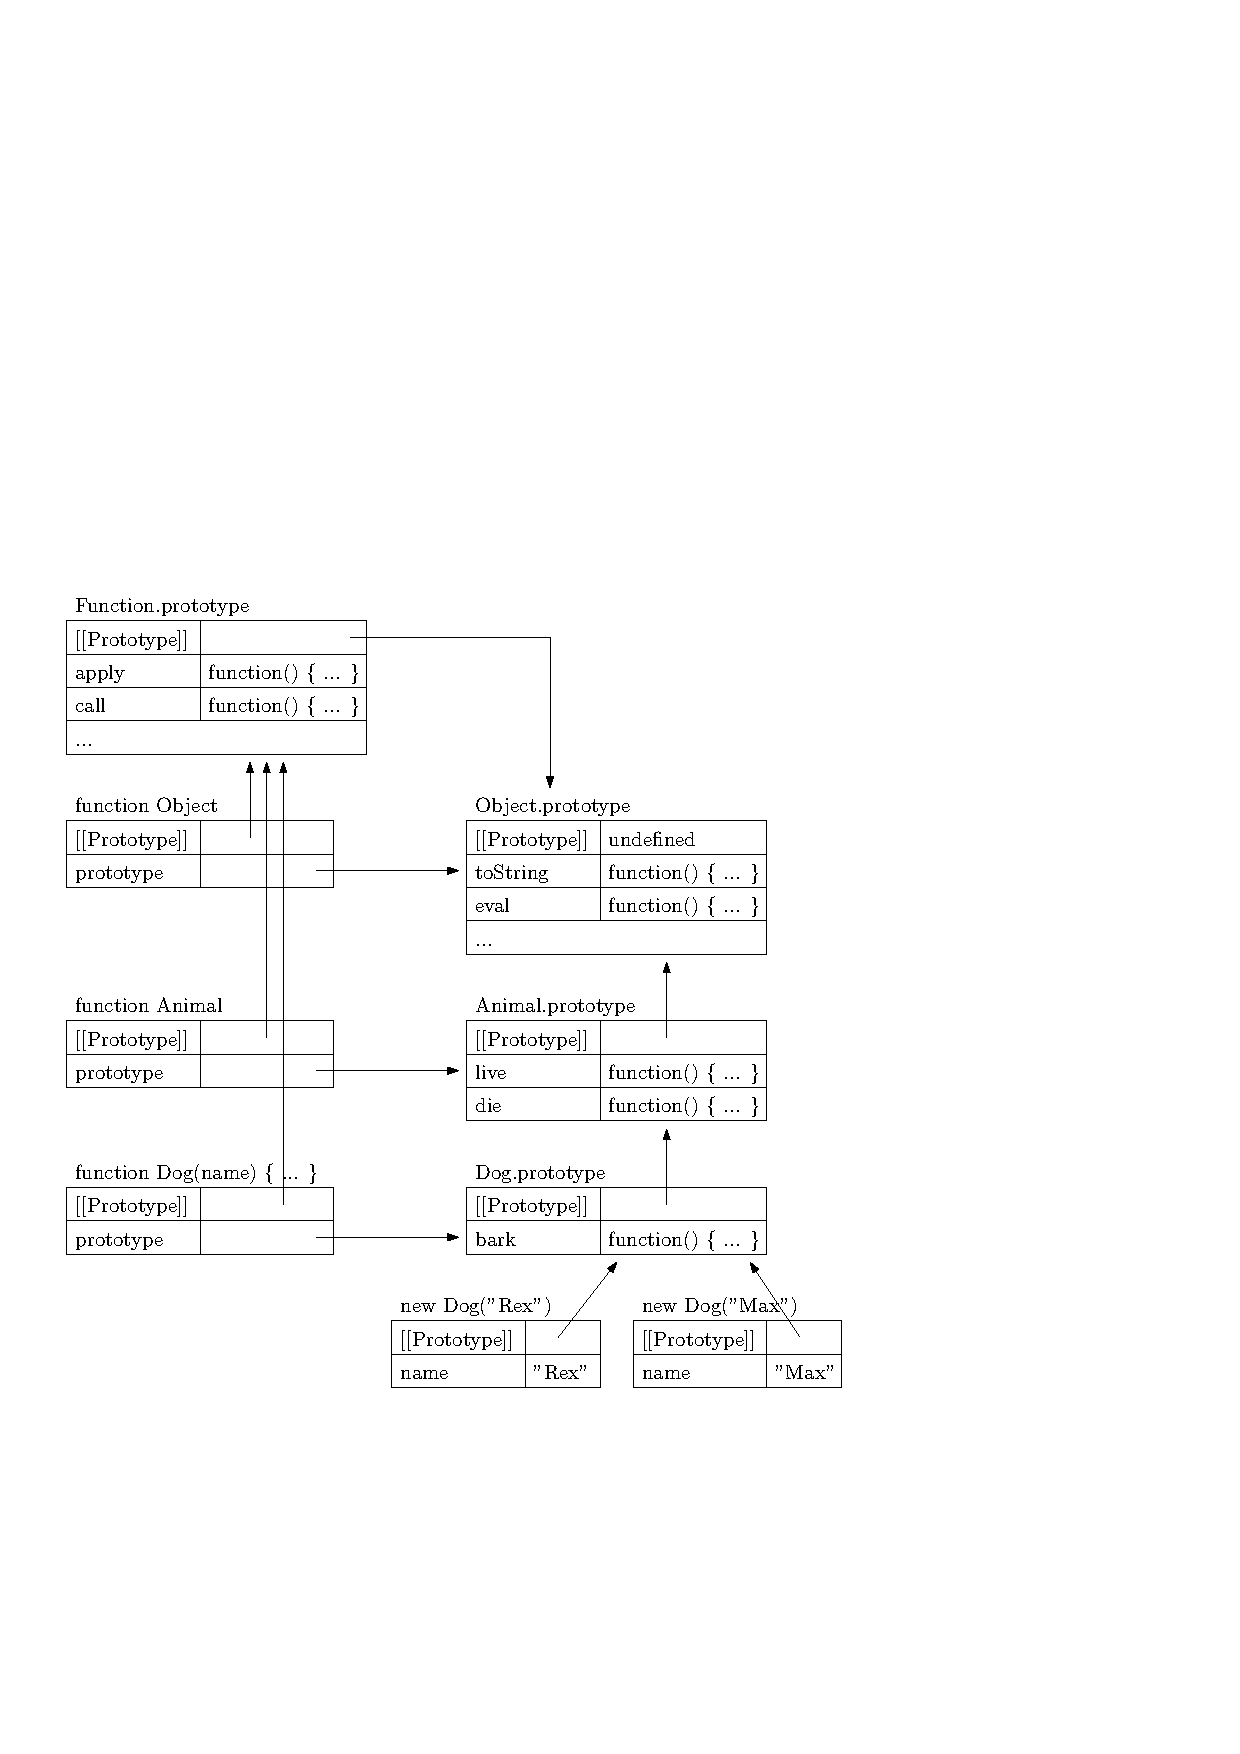
\includegraphics{img/JavaScriptPrototypes.pdf}
	\caption{JavaScript prototypes, cosntructors and instances.}
	\label{JavaScriptInheritance}
\end{figure}

The first thing to notice is, that all objects (and also functions because functions are objects) have the \texttt{[[Prototype]]} property which holds their prototypes. When a property of an object is being accessed, direct properties of the object are inspected first. If there is no direct property of the specified name, properties of the prototype are inspected. And so on until the prototype of currently inspected object is undefined. As a consequence, it behaves like if the object inheritted all properties of its prototype. The \texttt{[[Prototype]]} property is internal, does not change, is assigned once when the object is constructed and can not be changed programmatically.

So for example all functions inherit methods \texttt{apply} and \texttt{call} from their common prototype \texttt{Function.prototype} and transitively methods \texttt{toString} etc. from their prototype's prototype \texttt{Object.prototype}.

In order to create objects, a constructor function has to be defined first (e.g. the function \texttt{Animal} for animals). A constructor function may access the object that is being created via the \texttt{this} keyword and set some of its properties (e.g. the constructor function \texttt{Dog} sets \texttt{name} of a new dog). Moreover it may have associated special object in the property \texttt{prototype} that will be assigned as the \texttt{[[Prototype]]} to all objects created with the constructor function. If the function does not have the \texttt{prototype} specified, the standard \texttt{Object.prototype} is assigned to the created objects. Finally a new object is created by calling a constructor function together with the \texttt{new} keyword, e.g. \texttt{new Animal()}.

To sum it up, the hierarchy on the picture~\ref{JavaScriptInheritance} is set up in the following manner:

\begin{enumerate}
\item Define a constructor function for animals - the function \texttt{Animal}.
\item Assign a new object with properties \texttt{live} and \texttt{die} to the \texttt{prototype} property of the \texttt{Animal} function.
\item Define the dog constructor function \texttt{Dog} with body: \texttt{this.name = name;}.
\item Create a new \texttt{Animal} object (using \texttt{new Animal()}), define it's method \texttt{bark} and set it to the to the \texttt{prototype} property of the \texttt{Dog} function.
\item Create the dogs using \texttt{new Dog("Rex")} and \texttt{new Dog("Max")}.
\end{enumerate}

\paragraph{Environment} JavaScript is an interpreted language, therefore it requires a runtime evironment that interprets it and provides objects and functions for the programs interaction with the "outside world". In the context of web applications, both the runtime environment and the outside world is the web browser. The code is executed in a single thread which behaves similarly to an event loop. There is a queue of code that has to be executed. Code is enqueued to the queue from two main reasons: when a new script is loaded and when an external operation handled by the browser finishes and a callback has to be ivoked. The environment cyclically waits until the queue is non-empty and then sequentially executes everything in the queue. So it is quaranteed that nothing will run in parallel.

\section{Scala}

One of the best summaries of the Scala language is provided by its author himself, Martin Odersky, in \cite{ScalableComponents}:

\begin{quote}
"Scala fuses object-oriented and functional programming in a statically typed language. Conceptually, it builds on a Java-like core, even though its syntax differs. To this foundation, several extensions are added. From the object-oriented tradition comes a uniform object model, where every value is an object and every operation is a method invocation. From the functional tradition come the ideas that functions are First-class values, and that some objects can be decomposed using pattern matching. Both traditions are merged in the conception of a novel type system, where classes can be nested, classes can be aggregated using mixin composition, and where types are class members which can be either concrete or abstract."
\end{quote}

\paragraph{Style} The language is both imperative and functional, but tends and encourages to use rather the functional style. It supports most of the standard control structures known from e.g. Java. Adds some new control structures, the most important is the \texttt{match} statement (listing \ref{lst:MatchStatement}). Scala also generalizes and unifies existing control structures where it is possible: for cycles are abstracted into much more powerful \texttt{for} comprehensions (listing \ref{lst:ForComprehension}), multiple catch blocks are turned into one that matches against the catched exception (listing \ref{lst:CatchBlock}).

\begin{lstlisting}[frame=single,caption={Match statement.},label={lst:MatchStatement}]
list match {
   case Nil => "empty"
   case 'a' :: tail => "starts with 'a'"
   case (x: Int) :: _ if x > 3 => "starts with int > 3"
   case (x: Int) :: _ => "starts with int"
   case _ => "whatever"
}
\end{lstlisting}

\begin{lstlisting}[frame=single,caption={For comprehension.},label={lst:ForComprehension}]
for(e <- employees;
        if e.age > 25;
    c <- companies;
        if c.region == "DA";
        if c.name == e.companyName;
        difference = e.salary - c.avgSalary;
        if difference < 0		
) yield (e.name, c.name, difference)
\end{lstlisting}

\begin{lstlisting}[frame=single,caption={Catch block.},label={lst:CatchBlock}]
try {
    throwsException()
} catch {
    case _: IllegalArgumentException => println("argument")
    case _: IllegalStateException => println("state")
    case _: IOException => println("IO")
    case e => println(e.getMessage)
}
\end{lstlisting}

Scala does not differentiate between expressions and statements, because everything, that has been traditionally viewed as a statement (if-then-else, try-catch), has a return value. So for example a ternary operator is unnecessary, because if-else can be used instead (listing \ref{lst:IfElse}). There are many more features, for a thorough description refer to the Scala "bible" \cite{ScalaProgramming}.

\begin{lstlisting}[frame=single,caption={If-else as a ternary operator.},label={lst:IfElse}]
val result = if (a >= 0) "positive" else "negative"
\end{lstlisting}

\paragraph{Syntax} As it can be seen on the previous code samples, the syntax resembles Java or C\#, but is much more flexible while trying to reduce unnecessary clutter. It is possible to define methods, whose usage looks like built-in control structures, leave out parentheses or semicolons where possible etc. As a consequence, Scala is pretty suitable for design of domain specific languages. 

\paragraph{Type System} Unlike Java with distinct primitive and reference types, where the primitive types do not belong into the inheritance hierarchy, all Scala types inherit from the common ancestor \texttt{scala.Any}. The whole hierarchy is depicted on \ref{ScalaTypeSystem}, the types that are passed by value are descendants of the \texttt{scala.AnyVal}, reference types inherit from the \texttt{scala.AnyRef}. The only non-standard value type is the \texttt{scala.Unit} which represents a product of no types, i.e. 0-tuple. It has one inhabitant \texttt{()} and is for example used instead of the \texttt{void} keyword known from other languages.

\begin{figure}[ht]
  \centering
	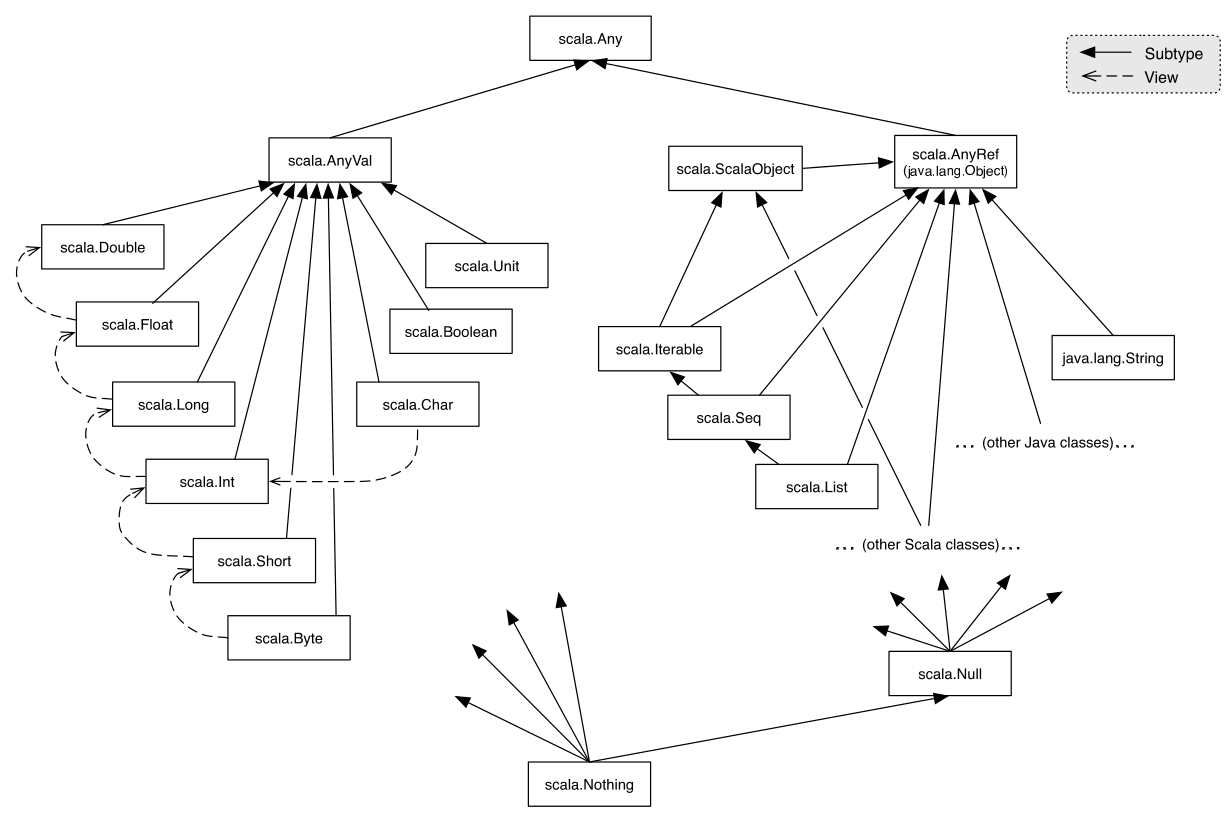
\includegraphics[width=\linewidth,height=\textheight,keepaspectratio]{img/ScalaTypeSystem.png}
	\caption{Scala Type System.}
	\label{ScalaTypeSystem}
\end{figure}

Note the \texttt{scala.Null} type with its only inhabitant \texttt{null} and the uninhabited type \texttt{scala.Nothing} (in type theory known as zero type). With them, it is always feasible to determine common supertype and common subtype for each two types\footnote{A common supertype is needed when inferring type of an expression that returns either type A or type B, a common subtype when unifying two generic types with type parameters on a contravariant position.}.

The types may take other types as parameters (known as generic types), the type parameters can be annotated with variance annotations (invariant, covariant, contravariant) and bounded (e.g. the type parameter has to be subtype of type X). Also some more advanced possibilities are supported - existential types, path-dependent types, structural types, etc\cite{ScalaAdvancedTypes}.

\paragraph{Functional Programming} Scala also supports a lot of features that can be found only in functional lanugages, so it is possible to write Scala programs solely in the functional style. But not purely, because mutable variables, which violate the referential transparency, are allowed. The most important functional concepts are:

\begin{itemize}
\item Closures - anonymous functions that capture the declaration site scope.
\item Immutable variables (\texttt{val}s).
\item Lazy evaluation of variables, function parameters or object fields.
\item Higher-order and nested functions.
\item Currying and partial application.
\item Pattern matching.
\item Tuples and algebraic data types.
\end{itemize}

\paragraph{Object Oriented Programming} On the other hand, Scala is a pure OO language, meaning that every value is an object. A data type may be declared either as a class, a trait or a singleton object. Classes are quite similar to Java classes, but on top of class inheritance, they may mix-in any amount of traits. Traits are basically enhanced Java interfaces with possibility to also define implementation. From the Scala perspective, the only difference between traits and classes is, that traits cannot have parametrized constructors.

The \texttt{static} fields and methods known from mainstream languages are not supported because it is difficult to abstract over them. To fill the gap, singleton objects behave like classes whose only instance is created during the class-loading process. They serve the purpose of static classes but may also inherit or mix-in other types and possibly override something, which isn't doable in languages that use the \texttt{static} modifier.

The famous diamond inheritance problem that always emerges with the multiple inheritance is solved using the technique called linearization\cite{Linearization}. Linearization is a deterministic process that specifies a single linear order for all of the type ancestors (i.e. all classes in the superclass chain and parent chains of all traits). Method resolution takes advantage of it and works in the linearization order, so there is no place for ambiguity left.

\section{Scala Compiler}
\label{sec:ScalaCompiler}

In the context of the thesis, it is also important to know how the scala compiler works, because it may be used by the Swat as a library for tasks that are specific for Scala compilation, but not that relevant from the Scala to JavaScript compilation perspective. The compiler architecture is summarized by Martin Odersky in \cite{ScalableComponents}:

\begin{quote}
"The Scala compiler, \texttt{scalac}, consists of several phases. The first phase is syntax analysis, implemented by a scanner and a conventional recursive descent parser. The result of this phase is an abstract syntax tree. The next phase attributes the syntax tree with symbol and type information. This is followed by a number of phases that transform the syntax tree. Most transformations replace some high-level Scala-specific constructs with lower-level constructs that can more directly be represented in bytecode. Other transformations perform optimizations such as inlining or tail call elimination. Transformations always consume and produce attributed trees."
\end{quote}

So the compiler can be understood as a sequence of phases where each phase takes an abstract syntax tree (AST) as its input from the previous phase, adds attributes to the AST or modifies the AST and passes the modified tree to the consequent phase.

In order to represent a scala program in the compiler, a couple of data structures needs to be defined\cite{Reflection}
. \texttt{Name}s represent identifiers that appear in the source code, e.g. class names or field names. \texttt{Symbol}s are used to bind a name and the entity it refers to, such as a class or a method. Anything that can be given a name has a symbol associated with it. Instances of the \texttt{Type} class represent information about the type of a corresponding symbol (the information include member methods, fields, base types etc). Finally, the ASTs are represented by \texttt{Tree} and its subclasses that correspond to various source code elements such as class definitions (\texttt{ClassDef}), method invocations (\texttt{Apply}) or if-else statements (\texttt{If}).

The only up-to-date description of the phases, the scalac consists of, can be found in the source code (class \texttt{scala.tools.nsc.Global}). Here are the most important ones:

\begin{description}[style=multiline,leftmargin=5cm]
\item[\texttt{syntaxAnalyzer}] Parses source code into ASTs, performs simple desugaring.
\item[\texttt{analyzer.namerFactory}] Parses source code into ASTs, performs simple desugaring.
\item[\texttt{analyzer.typerFactory}] Assigns types to symbols, the most complex phase.
\item[\texttt{patmat}] Converts the \texttt{match} expressions into if-else statements, labels and jumps.
\item[\texttt{uncurry}] Performs the opposite of currying, trnasforms variadic parameters to sequences, converts closures to anonymous classes and a lot of other similar, rather simple, operations. 
\item[\texttt{explicitOuter}] For each nested class, adds a field for the reference to the outer class instance. 
\item[\texttt{erasure}] Erases generic types, adds interfaces for traits.
\item[\texttt{lazyVals}] Converts lazy fields into methods.
\item[\texttt{constructors}] Moves field initialization into constructors.
\item[\texttt{mixer}] Performs the mix-in composition.
\item[\texttt{cleanup}] Platform specific cleanup.
\item[\texttt{deadCode}] One of many optimization phases, eliminates dead code.
\item[\texttt{jvm}] Generates the Java bytecode.
\end{description}



%%%%%%%%%%%%%%%%%%%%%%%%%%%%%%%%%%%%%%%%%%%%%%%%%%%%%%%%%%%%%%%%%%%%%%%%%%%%%%%%
\chapter{Analysis}

This chapter proposes, how some of the defined goals can be fulfilled, while providing more possibilities with their pros and cons. It should not be biased by the fact, that the source language is Scala, so the described methods could be applied even in a different environment. But for example purposes, Scala will be used, because it is the source language of the Swat. Moreover, this chapter elaborates on which of the proposed approaches is used by the Swat and why.

\section{Setup}

Compiler architecture has throughout years converged to a data flow consisting of canonical components. The source code is consumed by a scanner, that performs lexical analysis and produces a stream of lexical tokens. A parser takes the token stream on the input, performs syntactical analysis and builds up the ASTs. The ASTs are then processed by a semantical analyzer which validates them, assigns types to symbols and possibly transforms the ASTs. These three components are marked as the frontend components. When the abstract syntax trees leave the frontend, they go to a backend, which is resposnible for generation of the target language/assembly/byte code. The backend usually consists of several subcomponents that firstly produce some intermediate code, optimize it and then generate the machine specific code. Such a data flow can be seen on the top part of the pricture \ref{Compiler}.

\begin{figure}[ht]
  \centering
	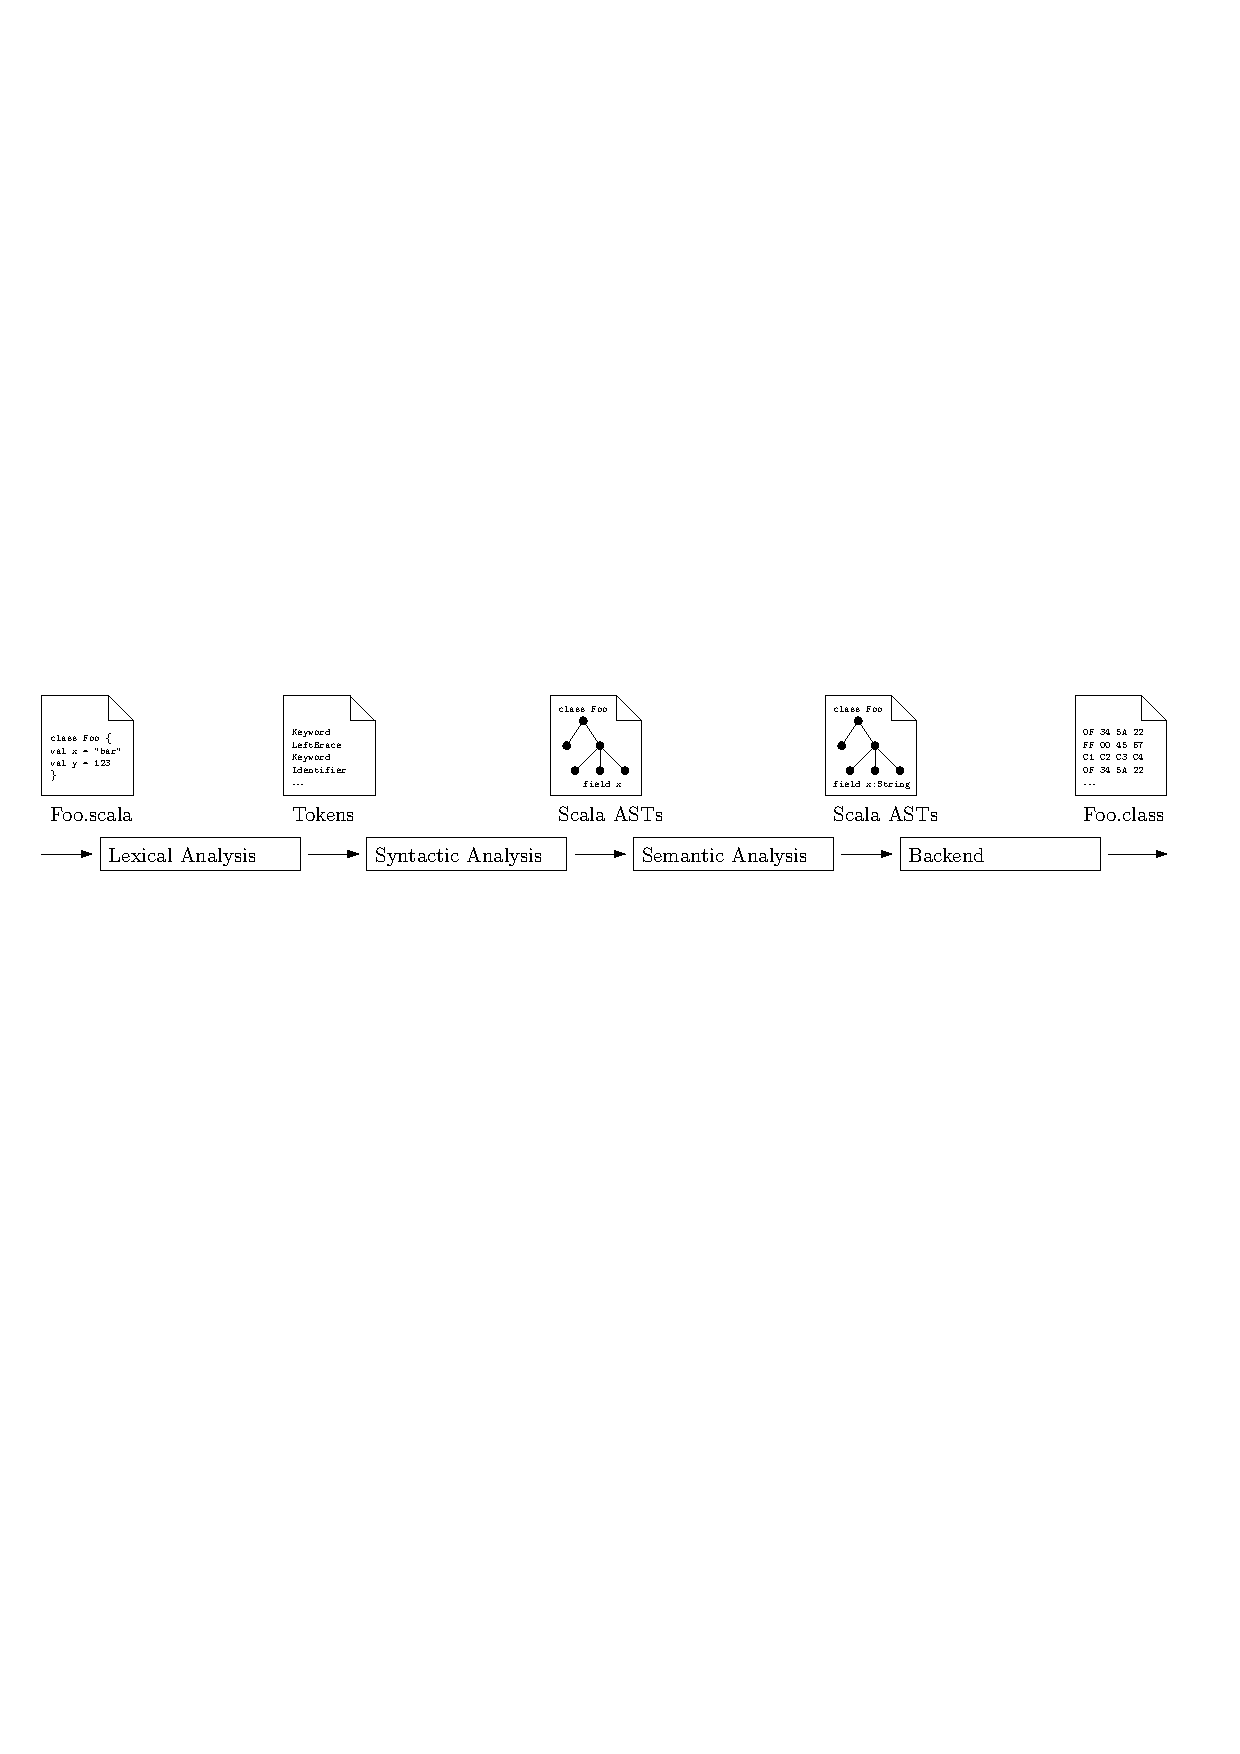
\includegraphics[width=\linewidth,height=\textheight,keepaspectratio]{img/Compiler.pdf}
	\caption{Compiler architecture}
	\label{Compiler}
\end{figure}

In order to transform programs to JavaScript, one needs to work with them programmatically. ASTs exactly serve this purpose and because standard compilers (e.g. javac, csc, scalac) already handle the transformation from source code to ASTs, reusing that functionality is definitely the way to go. The standard compiler architecture offers few places where the ASTs can be obtained. As depicted on the figure \ref{Compiler}, it is either before the semantic analysis (option A) or after the semantic analysis (option C). If the compiler components are subdivided into phases, it may be even possible to access the syntax trees in the middle of the sematic analysis (option B). That mostly depends on architecture of the source language compiler, whether it allows such an interception.

Choice of the point when the ASTs are obtained determines abilities of the JavaScript frontend to some extent. Before the semantic analysis, the abstract syntax trees just mirror the source code and do not contain any added deduced information. After the analysis, the program is on one hand proven correct and e.g. all the variables have known type. On the other hand, some particular ASTs may be oversimplified and desugared, even if the original trees are directly expressible in JavaScript (for example closure desugaring to anonymous classes). If the semantic analysis is sequential, it is possible to access the ASTs after each phase and thus have wider range of choices.

The JavaScript frontend is responsible for creation of JavaScript ASTs that correspond to the input Scala ASTs. It may use different approaches to tackle its task. One option is to construct the JavaScript ASTs utilizing only JavaScript language primitives and internal functions, so the resulting code would be executable as it is. The other way is to move some of the logic to a JavaScript runtime library, so the outputted JavaScript code would run only if the runtime library is present in the global scope. The two approaches are illustrated on how the Scala snippet \ref{lst:ScalaComVsRun} could be compiled to JavaScript - listings \ref{lst:JsCompileTime} and \ref{lst:JsRunTime}.

\begin{lstlisting}[frame=single,caption={Scala input.},label={lst:ScalaComVsRun}]
lazy val foo = reallyLongOperation()

// Causes evaluation of foo.
val bar = foo 
\end{lstlisting}

\begin{lstlisting}[language=JavaScript,frame=single,caption={Compile-time option outcome.},label={lst:JsCompileTime}]
var foo_value = undefined;
var foo = function() {
  if (typeof foo_value === "undefined") {
    foo_value = reallyLongOperation();
  }
  return foo_value;
};

var bar = foo();
\end{lstlisting}

\begin{lstlisting}[language=JavaScript,frame=single,caption={Runtime option outcome.},label={lst:JsRunTime}]
// runtime.lazy is a library function.
var foo = runtime.lazy(function() {
  return reallyLongOperation();
});

var bar = foo();
\end{lstlisting}

After the JavaScript frontend, which may itself consist of multiple phases, comes the JavaScript backend. It generates JavaScript code corresponding to the ASTs and may optimize the output either by itself or by an external tool (Google Closure compiler\cite{GoogleClosure} is the most popular).

In the Swat, initial decision was to produce JavaScript code that would resemble Scala as much as possible and use just the compiler phases that analyze the code (\texttt{syntaxAnalyzer}, \texttt{analyzer.namerFactory}, \texttt{analyzer.typerFactory}). The motivation behind that was to simplify debugging of the compiled code in a web browser. But it turned out that it would be a lot work to implement JavaScript runtime counterparts of Scala control structures that are not present in JavaScript. Moreover, it would be beneficial to execute some of the latter phases before Swat, however Scala compiler phases have fixed order and dependencies and it is not possible left out a phase from the sequence. 

So the resulting solution is a compromise between "similarity to Scala" and "reimplementation of what the latter phases do". This can be illustrated on the \texttt{patmat} phase which desugars \texttt{match} expressions into sequences of conditions. Not using \texttt{patmat} would basically mean to reimplement in on the JavaScript runtime level. The phase \texttt{erasure} has been chosen as the one the Swat will run before. From the top level point of view, the phases that somehow modify method bodies or parameters are executed before Swat. The phases that operate on the class level (e.g. transform traits into class and interface pairs, perform the mix-in composition) run after the Swat.

A disadvantage is that the resulting code sometimes does not resemble the source Scala code, which means that debugging in the browser is tricky. Solution for this issue are source maps\cite{SourceMaps} that establish mapping between the executed JavaScript code (minified, compiled) and the original code (not minified, even possibly not JavaScript) and allow an user to debug the original code.

In order to minimize size and bilerplate in the produced JavaScript and to increase its readability, the Swat JavaScript fronted counts with a runtime library and tries to move functionality there if it is both possible and beneficial. In cases when the compile-time option nor the runtime option is apparently better than the other, the runtime option is chosen, because modifying the runtime is by far simpler than modifying the compiler.

\section{Interoperation with JavaScript}

One of the crucial requirements of a compiler targetting JavaScript is enabling the programs written in a source language to interoperate with the JavaScript environment. Inherent restriction is, that the used solution should not violate syntax of the source language. The following three ways turned out to be the most usable and moreless orthogonal to each other: 

\begin{description}
\item[Annotations] A method or a field is annotated with an annotation that takes JavaScript code as the only string parameter. When the compiler encounters a method AST or a field AST that is annotated with such annotation, it simply ignores the field value or method body and instead uses the JavaScript code stored in the annotation.
\item[Adapters] For all the JavaScript APIs and objects that should be usable from the source language, so called "adapter" classes are defined in the source language. They should exactly match the JavaScript definitions in terms of names, fields, methods, parameters etc. and should be marked with an annotation in order to be distinguishable. They do not have to be implemented, but the type signatures should match the specification. When the compiler encounters such an adapter class, it knows that it is something that is already present in the JavaScript environment, so it can be completely ignored. 
\item[Dynamic] This option is relevant only to source languages that support the concept of a dynamic class. In Scala, one would define an object representing the JavaScript global scope: \texttt{object global extends Dynamic}. The object mixes-in the \texttt{scala.Dynamic}\cite{ScalaDynamic} trait, so any field can be selected or any method can be invoked on that particular object. For example \texttt{global.window} will be turned by the Scala compiler before the typing phase into \texttt{global.selectDynamic("window")}. Such an invocation can later be transformed by the JavaScript frontend into \texttt{window}.
\end{description}

All three approaches are presented on the listing \ref{lst:Interoperation}. The JavaScript output would be same for each of them.

\begin{lstlisting}[frame=single,caption={Scala interoperation options.},label={lst:Interoperation}]
// Annotations.
@native("window.document")
val document1: Any = null

// Adapters.
@adapter class Document {
  // ...
}
@adapter object window {
  val document: Document = null
  // ...
} 
val document2: Document = window.document

// Dynamic.
val document3: Any = global.window.document
\end{lstlisting}

As it was mentioned in the motivation, static typing is an advantage in the context of large applications, so the option {\it Adapters} is the preferred one. Unlike the two other, it preserves type safety. The tradeoff is that it is uncomparably more time-consuming compared to the other options. The {\it Annotations} and {\it Dynamic} provide similar functionality, but should be used as a last resort only if the {\it Adapters} are not applicable. Swat uses and favors the {\it Adapters} and for the exceptional cases the {\it Annotations} which are little bit more flexible than the {\it Dynamic} option.

\section{Frontend}

A heart of the whole toolkit is the JavaScript frontend responsible for transformation of source language AST to JavaScript ASTs. It starts given the whole program (or its top level part) in the form of a syntax tree, traverses the AST and produces JavaScript ASTs. According to the current subtree, whose root the fronted is  visitng, it should produce JavaScrit counterpart for that subtree. The following sections describe, how particular tree types should be represented in JavaScript. It is natural to start with the top-level ASTs that encapsulate everything else and traverse down the tree through class definitions, their member definitions to the simplest expressions on the leaf level of the tree.

\subsection{Scope of a Compilation Unit}

The top level tree type represents a compilation unit (one source file) and it contains possibly nested definitions of packages. The package definitions are usually non-empty, they encapsulate type definitions (definitions of classes, objects and traits).

Important decision on this level is, whether the whole compilation unit should be transformed into one JavaScript AST which would be consequently turned by the JavaScript backend into one JavaScript file. Or whether the compilation unit should be somehow splitted into multiple files. An inspiration can be found in the standard Scala compiler which splits the compilation unit into type definitions and produces separate classfiles (\texttt{*.class}) for each type definition.

For a compiler targetting JavaScript, the splitting opens up a possibility, to track and store dependencies of each type definition together with its outputted JavaScript typefile (analogue to a Java classfile). A dependency is either an instantiated class, an accessed singleton object, an used type or a supertype of the type definition. With this information, the JavaScript typefiles form an oriented dependency graph. It would also be possible to track dependencies among compilation units, however it wouldn't be any advantage over dependencies among type definitions and wouldn't be as transparent either.

The entry point to an application, in the Scala environment, is a singleton object that mixes-in the \texttt{scala.App} trait, in other languages it is a static class. But not all web applications are in the form of a single page. It is quite common that there are multiple pages with different functionality, therefore the application has multiple entry-points corresponding to the different pages. 

So in order to run an application on a page, a typefile corresponding to the entry point has to be loaded with all its transitive dependencies. If the particular entry point has just a few dependencies, then the size of the resulting JavaScript, that has to be downloaded by the client, is small. Even though the whole project may consist of hundreds of classes. The same applies for external libraries. If a library is structured in the same manner (typefiles with dependencies) and the application uses just a fraction of the library, then resulting JavaScript still stays small.

For Swat, extracting all type definitions from the compilation unit and producing standalone typefiles for each of them is a necessity, because the Scala standard library\cite{ScalaLibrary}, which is an implicit dependency of all Scala programs, contains thousands of classes. Having the library packed in a single file whose size would exceed megabytes wouldn't be acceptable in any real-world usage scenario. 

\subsection{Types}

As the compilation unit handling is sorted out, it now comes to how the type definitions should be represented in JavaScript. Packages or namespaces are not an issue because solution for them is pretty straightforward (illustrated on the listing \ref{lst:JavaScriptPackages}).

\begin{lstlisting}[language=JavaScript,frame=single,caption={Packages in JavaScript.},label={lst:JavaScriptPackages}]
// Declaration of the package "foo.bar.baz".
var foo = {};
foo.bar = {};
foo.bar.baz = {};

// Definition of types in the package.
foo.bar.baz.Animal = {
  // ...
};

foo.bar.baz.Dog = {
  // ...
};
\end{lstlisting}

\begin{itemize}
\item Inheritance, solving static initialization order, encoding type information.
\end{itemize}

\subsection{Scope of a Type}

\begin{itemize}
\item Extracting members.
\item Processing fields, nothing has to be declared in JS, therefore setting initial values in constructor is enough, lazy fields.
\item Processing methods, taking care of overloading and constructor.
\end{itemize}

\subsection{Expression Scope}

\begin{itemize}
\item Scoping, var self = this.
\item Primitive types, their representation in JavaScript, decision not to extend JavaScript built-in objects, primitive type methods as extension methods or operators.
\item Anonymous functions, partial functions.
\item Method invocation, super call, this call, Any type methods as internal swat methods.
\item Local methods and types.
\item Control structures.
\end{itemize}

\section{Library Distribution}

Storing the compiled JavaScript files as resources of the very same module, so they're included in the packaged jar together with the Java classfiles. Integration of such library and using it on both platforms is therefore simple. Implies need of a type loader, that can access the type files.

\section{Runtime}

The only interesting thing, from the analysis point of view, is encoding class/trait inheritance in JavaScript using the object prototype chaining.



%%%%%%%%%%%%%%%%%%%%%%%%%%%%%%%%%%%%%%%%%%%%%%%%%%%%%%%%%%%%%%%%%%%%%%%%%%%%%%%%





%%%%%%%%%%%%%%%%%%%%%%%%%%%%%%%%%%%%%%%%%%%%%%%%%%%%%%%%%%%%%%%%%%%%%%%%%%%%%%%%
\chapter{Implementation}

\section{Environment}

Prerequisities, Scala, versions, build tools.

\section{Project Overview}

The big picture of the whole project, interaction of all components and description of the processes in it so one can get understanding of how the whole thing works, including the type loading, RPC and JSON serializers.

\section{API \& Adapters}

Description of the annotations: ignored, adapter, native, dependency. Walkthrough (or rather example) on how to create adapters without the necessity to blindly copy the specification using traits as shared interfaces.

\section{Compiler}

Basically a big match against all types of Scala ASTs that follows the principles described in analysis.

\subsection{Build Process}

Integration to SBT.

\section{Runtime}

\subsection{Client}

Description of everything intereseting in the swat.js.

\subsection{Standard Libraries}

Lazy approach, modifying the sources to exclude parts not relevant in the JavaScript environment. The purpose is not to blindly port everything but rather only a portion which is usable in JavaScript.

\subsection{Type Loader}

How it works on the server side and how on the client side.

\subsection{JSON Serializer}

The format that enables us to serialize even graphs of objects with cyclic references. Including type information in order to succesfully deserialize on the server and assign proper prototype on the client.

\subsection{RPC}

Support from the compiler, thin client proxy and server dispatcher. Only non-blocking, utilizing Scala Futures and Promises, exception handling.

\section{Integration with a Web Framework}

Should be as simple as possible, Play Framework example.

\section{Tests}



%%%%%%%%%%%%%%%%%%%%%%%%%%%%%%%%%%%%%%%%%%%%%%%%%%%%%%%%%%%%%%%%%%%%%%%%%%%%%%%%
\chapter{Comparison with Similar Tools}

The tools at the time of thesis start (ScalaGWT, s2js, scalosure) and current scala-js, js-scala.



%%%%%%%%%%%%%%%%%%%%%%%%%%%%%%%%%%%%%%%%%%%%%%%%%%%%%%%%%%%%%%%%%%%%%%%%%%%%%%%%
\chapter{Conclusion}

\section{Critical Evaluation}

What was done, what lacks the most (Scala library), but stating that everything got done to some extent. Discussion about the overloading problem and the taken decision.

\section{Roadmap}

Actually the main purpose and goal is to really simplify tasks, that aren't programmer friendly in JavaScript. The grounds have been laid, so the really interesting applications can be now implemented. Some of the interesting directions are described in the following sections.

\subsection{Web workers}

Actor like abstraction over web workers, with help of JSON serializer and type-loader.

\subsection{Template engine}

Problems with JavaScript templating and how it could be solved using string interpolation.

\subsection{Build process}

Swat as a SBT plugin, resident compilation that would simplify the development process.



%%%%%%%%%%%%%%%%%%%%%%%%%%%%%%%%%%%%%%%%%%%%%%%%%%%%%%%%%%%%%%%%%%%%%%%%%%%%%%%%
\def\bibname{Bibliography}

\begin{thebibliography}{99}
\addcontentsline{toc}{chapter}{\bibname}

\bibitem{Flash}
	Introducing the Adobe Flash Platform.\\
	http://www.adobe.com/devnet/flashplatform/articles/flashplatform\_overview.html
	
\bibitem{JavaApplets}
	Java applet.\\
	http://en.wikipedia.org/wiki/Java\_applet
	
\bibitem{JavaScript}
	JavaScript.\\
	http://en.wikipedia.org/wiki/JavaScript
	
\bibitem{EcmaScript}
	{\sc Ecma} International.\\
	ECMAScript Language Specification.\\
	http://www.ecma-international.org/publications/files/ECMA-ST/Ecma-262.pdf
	
\bibitem{Ajax}
	{\sc Garrett,} Jesse James.\\
	Ajax: A New Approach to Web Applications.\\
	http://www.adaptivepath.com/ideas/ajax-new-approach-web-applications

\bibitem{Html5}
	HTML5 Introduction.\\
	http://www.w3schools.com/html/html5\_intro.asp

\bibitem{Backends}
  {\sc Ashkenas,} Jeremy.\\
  List of languages that compile to JS.\\
  https://github.com/jashkenas/coffee-script/wiki/List-of-languages-that-compile-to-JS
	
\bibitem{Meijer}
	{\sc Meijer,} Erik and {\sc Drayton,} Peter.\\
	Static Typing Where Possible, Dynamic Typing When Needed: The End of the Cold War Between Programming Languages.\\
	http://research.microsoft.com/en-us/um/people/emeijer/Papers/RDL04Meijer.pdf
	
\bibitem{RequireJs}
	RequireJS.\\
	http://requirejs.org/
	
\bibitem{HeadJs}
	HeadJS.\\
	http://headjs.com/
	
\bibitem{JsLint}
	JSLint, The JavaScript Code Quality Tool.\\
	http://www.jslint.com/
	
\bibitem{JsHint}
	JSHint, a JavaScript Code Quality Tool.\\
	http://www.jshint.com/

\bibitem{GoogleClosure}
	Google Closure Compiler.\\
	http://closure-compiler.appspot.com/home
	
\bibitem{Dart}
	Dart: Structured web apps.\\
	www.dartlang.org/
	
\bibitem{CoffeeScript}
	CoffeeScript.\\
	http://coffeescript.org/
	
\bibitem{TypeScript}
	TypeScript.\\
	www.typescriptlang.org/
	
\bibitem{NodeJs}
	node.js\\
	http://nodejs.org/
	
\bibitem{Rpc}
	Remote procedure call.\\
	http://en.wikipedia.org/wiki/Remote\_procedure\_call
	
\bibitem{Gwt}
	GWT Project.\\
	www.gwtproject.org/
	
\bibitem{SharpKit}
	SharpKit - C\# to JavaScript Compiler.\\
	http://sharpkit.net/
	
\bibitem{Tiobe}
	TIOBE Programming Community Index for July 2013.\\
	http://www.tiobe.com/index.php/content/paperinfo/tpci/index.html
	
\bibitem{Dom}
	Document Object Model (DOM) Specifications.\\
	http://www.w3.org/DOM/DOMTR
		
\bibitem{Jquery}
	jQuery.\\
	http://jquery.com/
	
\bibitem{Sbt}
	Scala Build Tool.\\
	http://www.scala-sbt.org/
	
\bibitem{Play}
	Play.\\
	http://www.playframework.com/
	
\bibitem{Typesafe}
	Typesafe.\\
	http://typesafe.com/
	
\bibitem{Self}
	Self.
	http://selflanguage.org/
	
\bibitem{ScalableComponents}
	{\sc Odersky,} Martin and {\sc Zenger,} Matthias.\\
	Scalable Component Abstractions.\\
	http://lampwww.epfl.ch/~odersky/papers/ScalableComponent.pdf
	
\bibitem{Linq}
  LINQ (Language-Integrated Query).\\
  http://msdn.microsoft.com/en-us/library/vstudio/bb397926.aspx
	
\bibitem{ScalaProgramming}
	{\sc Odersky,} Martin and {\sc Spoon,} Lex and {\sc Venners,} Bill.\\  Programming in Scala, Second Edition.\\
	Artima, 2010
	
\bibitem{ScalaAdvancedTypes}
	Advantages of Scala's Type System.\\
	http://stackoverflow.com/questions/3112725/advantages-of-scalas-type-system
	
\bibitem{Linearization}
  {\sc McBeath}, Jim.\\
	Scala Class Linearization.\\
	http://jim-mcbeath.blogspot.cz/2009/08/scala-class-linearization.html
	
\bibitem{Reflection}
	Symbols, Trees, and Types.\\
	http://docs.scala-lang.org/overviews/reflection/symbols-trees-types.html
	
\bibitem{SourceMaps}
  {\sc Seddon,} Ryan.\\
	Introduction to JavaScript Source Maps.\\
  http://www.html5rocks.com/en/tutorials/developertools/sourcemaps/
	
\bibitem{W3c}
  World Wide Web Consortium.\\
	http://www.w3.org/
	
\bibitem{ScalaDynamic}
  Scala Dynamic.\\
	http://www.scala-lang.org/api/current/index.html\#scala.Dynamic
	
\bibitem{ScalaLibrary}
	Scala Standard Library API.\\
  http://www.scala-lang.org/api/current/index.html\#package
	
\bibitem{Lazy}
  Lazy initialization.\\
	http://en.wikipedia.org/wiki/Lazy\_initialization
	
\bibitem{CompilerPlugins}
  Writing Scala Compiler Plugins.\\
  http://www.scala-lang.org/node/140
	
\bibitem{ScalaFutures}
  Futures and Promises.\\
  http://docs.scala-lang.org/overviews/core/futures.html
	
\bibitem{ScalaGwt}
  Scala+GWT Project.\\
  https://github.com/scalagwt
	
\bibitem{S2js}
  S2JS Compiler Plugin.\\
  https://github.com/alvaroc1/s2js
	
\bibitem{Scalosure}
  Scalosure.\\
  https://github.com/efleming969/scalosure
	
\bibitem{JsScala}
  js.scala: JavaScript as an embedded DSL in Scala.\\
  https://github.com/js-scala/js-scala
	
\bibitem{ScalaJs}
  Scala.js, a Scala to JavaScript compiler.\\
  https://github.com/sjrd/scala-js
	
\bibitem{WebWorkers}
  Using web workers.\\
  https://developer.mozilla.org/en-US/docs/Web/Guide/Performance/Using\_web\_workers
	
\bibitem{Actors}
  Actor Model.\\
  http://en.wikipedia.org/wiki/Actor\_model
	
\bibitem{Akka}
	akka.\\
	http://akka.io/
	
\bibitem{WebSockets}
  Introducing WebSockets: Bringing Sockets to the Web.\\
	http://www.html5rocks.com/en/tutorials/websockets/basics/
	
\bibitem{StringInterpolation}
  Scala Documentation.\\
	String Interpolation.\\
	http://docs.scala-lang.org/overviews/core/string-interpolation.html
	
\bibitem{Equality}
  {\sc Odersky,} Martin and {\sc Spoon,} Lex and {\sc Venners,} Bill.\\
  How to Write an Equality Method in Java.\\
	{sc}
	http://www.artima.com/lejava/articles/equality.html
	
\end{thebibliography}





%%%%%%%%%%%%%%%%%%%%%%%%%%%%%%%%%%%%%%%%%%%%%%%%%%%%%%%%%%%%%%%%%%%%%%%%%%%%%%%%
\appendix
\appendixpage
\addappheadtotoc

\chapter{User Manual}

\chapter{Sample Application}

A nice example could be online SWAT compiler, that would let the user write some Scala code to a textarea, invoke the Swat compiler (through RPC on the server) and display the compiler code.



%%%%%%%%%%%%%%%%%%%%%%%%%%%%%%%%%%%%%%%%%%%%%%%%%%%%%%%%%%%%%%%%%%%%%%%%%%%%%%%%
\chapter{Content of attached CD}





\printnomenclature




\end{document}
